%% This is an example first chapter.  You should put chapter/appendix that you
%% write into a separate file, and add a line \include{yourfilename} to
%% main.tex, where `yourfilename.tex' is the name of the chapter/appendix file.
%% You can process specific files by typing their names in at the 
%% \files=
%% prompt when you run the file main.tex through LaTeX.
\chapter{Implementation}
This chapter revolves around intermediate code generation part of the compiler in which translation of the source program into target code takes place. In the process of translating a program written in a given language into code for a given target machine, a compiler typically constructs a sequence of intermediate representation which can have a variety of forms \cite{lam2006compilers}. High-level representations are close to the source language and low-level representations are close to the target machine. Syntax trees are one of the most commonly used form of high-level intermediate representation during syntax and semantic analysis. In this thesis, we do not create our own syntax trees representation but reuse the Scala Abstract Syntax Trees (AST) given freely by the Scala compiler's parser and type checker \cite{stocker2010scala}. 


\AK{Comment here!}


\begin{figure}[h!]
\centering
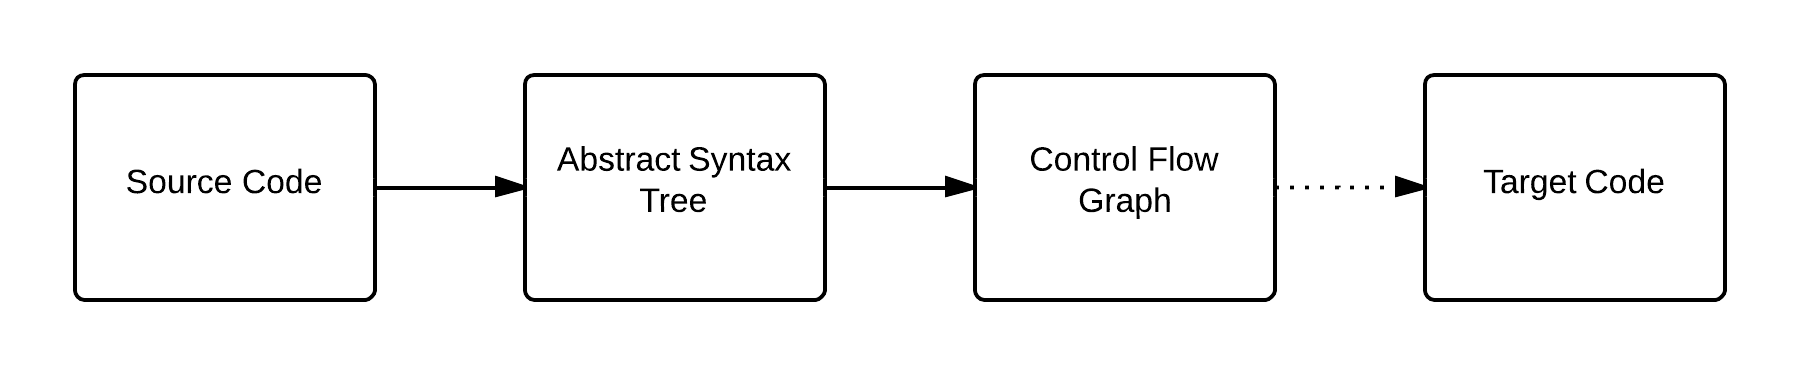
\includegraphics[width=0.8\linewidth]{figures/CompStructure}
\caption{Intermediate Representations}
\label{fig:Compiler}
\end{figure}

We divide the problem of translating the source program to target code into three stages. The first stage is to traverse the given AST and transform it to a more low-level intermediate representation which is Control Flow Graph (CFG); the steps are depicted in Figure 1.1. This thesis covers the design of the algorithm and implementation to transform the AST into CFG. A sample Scala program with control flow and iteration is presented in this chapter to show the process and result. The second stage is to analyze the CFG and identify the data dependencies between each block of the graph. In the end, we generate the executable code for the underlying system. The driver program of the WMS will then execute this code. The design of the algorithm and expected result of the last two stages are also delivered in this thesis. 

\section{Scala AST}
This section gives necessary introduction to AST to allow the reader to understand the transformation process from the source language to the target language. AST is one of the most important intermediate representations. During parsing, compiler creates syntax-tree nodes to represent significant programming constructs. As analysis continues, information is added to the node in the form of attributes associated to the node depending on the translation to be performed \cite{lam2006compilers}. In this thesis, we do not create our own AST representation but reuse the Scala compiler's parser and type checker. Additionally, the Scala compiler also provides a tool to traverse and transform an AST \cite{stocker2010scala}. 

Scala AST or Trees are the basis of abstract syntax which is used to represent programs. The Scala compiler uses AST as an intermediate representation before generating bytecode \cite{demarne2014scala}. In Scala reflection, Trees can be produced or used by the following APIs \cite{symboltreestypes}.

\begin{itemize}
\item Scala annotations. This API uses AST to represent their arguments and is exposed in \texttt{Annotation.scalaArgs}. 
\item \texttt{reify}. This special method takes an expression and returns an AST that represent this expression.
\item Compile time reflection with macros \cite{scalamacros} and runtime compilation with toolboxes use trees as their program representation medium. Macros expand trees at compile time allowing programmers to hack and manipulate AST within the compilation scope \cite{burmako2013scala}. 
\end{itemize} 

\subsection{AST Classes}
This section introduces some of the concrete trees classes that are used in traversing the trees in our implementation. All concrete classes are case classes, thus their parameters are listed following the class name as follows \cite{stocker2010scala}. 
\begin{itemize}
\item \texttt{Block(stats: List[Tree], expr: Tree)}. A Block consists of a list of statements and returns the value of expr.
\item \texttt{ValDef(mods: Modifiers, name: Name, tpt: Tree, rhs: Tree)}. Val- ue definitions are all definitions of vals, vars (identified by the MUTABLE flag) and parameters (identified by the param flag).
\item \texttt{LabelDef(name: Name, params: List[Ident], rhs: Tree)}. The Label- Def tree is used to represent iteration, both $While$ and $Do-While$ iteration. The Scala language specification \cite{odersky2004scala} defines that the while loop expression \texttt{while(e1) e2} is typed and evaluated as if it is an application of \texttt{whileLoop(e1)(e2)} where the hypothetical function \texttt{whileLoop} is defined in Listing 1.1 below. 
\begin{lstlisting}[language=scala,caption=WhileLoop Function, label = whileloop]
def whileLoop(cond: => Boolean)(body: => Unit): Unit = if (cond) { body ; whileLoop(cond)(body) } else {}
\end{lstlisting}
\item \texttt{Assign(lhs: Tree, rhs: Tree)}. Assign trees are used for non-initial assignments to variables. The lhs typically consists of an Ident(name) and is assigned the value of the rhs which normally contains an application (Apply) of a function. 
\item \texttt{If(cond: Tree, thenp: Tree, elsep: Tree)}. An If statement consists of three parts: the condition, the then part and the else part. If the else part is omitted, the literal () of type Unit is generated and the type of the conditional is set to an upper bound of Unit and the type of the then expression, usually Any.
\end{itemize}

\subsection{Generating Scala AST}
Scala macros is used in this thesis to lift the root Block of a Scala program into a monatic comprehension of intermediate representation. We present a sample Scala program with iteration and an If statement inside the iteration (refer to Listing 1.2) and show the generated Scala AST of the program. 
\\
\begin{lstlisting}[language=scala, caption=Workflow with Conditional, label = workflow2]
val e1 = DataSource("/tmp/input1.txt", CsvInputFormat[(String, Int, Int)]()).filter(x => x._1 == "Joshua")
val e2 = DataSource("/tmp/input2.txt", CsvInputFormat[(String, Int, Int)]()).filter(x => x._1 == "Marten")
var e3: DataSet[(String, Int, Int)] = null
var i = 0

while(i < 0) {
if (e1.map(x => x._2).reduce((x, y) => Math.max(x, y)).fetch().head > 50)
        e3 = e1.map { x => (x._1, x._2 + 1000, x._3)}
    else
    	e3 = e2.map { x => (x._1, x._2 + 1500, x._3)}
    }

val e4 = e3.write("/tmp/output.txt", CsvOutputFormat[(String, Int, Int)]())

e4
\end{lstlisting}

As shown in Scala AST in Figure 1.2, the program is represented by a Block which consists of list of statements and an expression which holds the final return value. Each of the variable definition is presented by a ValDef. The LabelDef in the AST represent the While statement in the program and consists of a name and a rhs of type If. The If statement consists of the three parts: condition, then part, and else part. In the while or LabelDef case, the else part which is of type Literal only contains an empty constant value. The then part is expanded to another list of statements and expression. Given that in the sample Scala program, there is a control flow inside the body of the loop, the statement then consists of another If statement. The then and else part of this If statement are of type Assign since in the program we assign a map function in the rhs to a variable name in the lhs. 

\begin{figure}[h!]
\centering
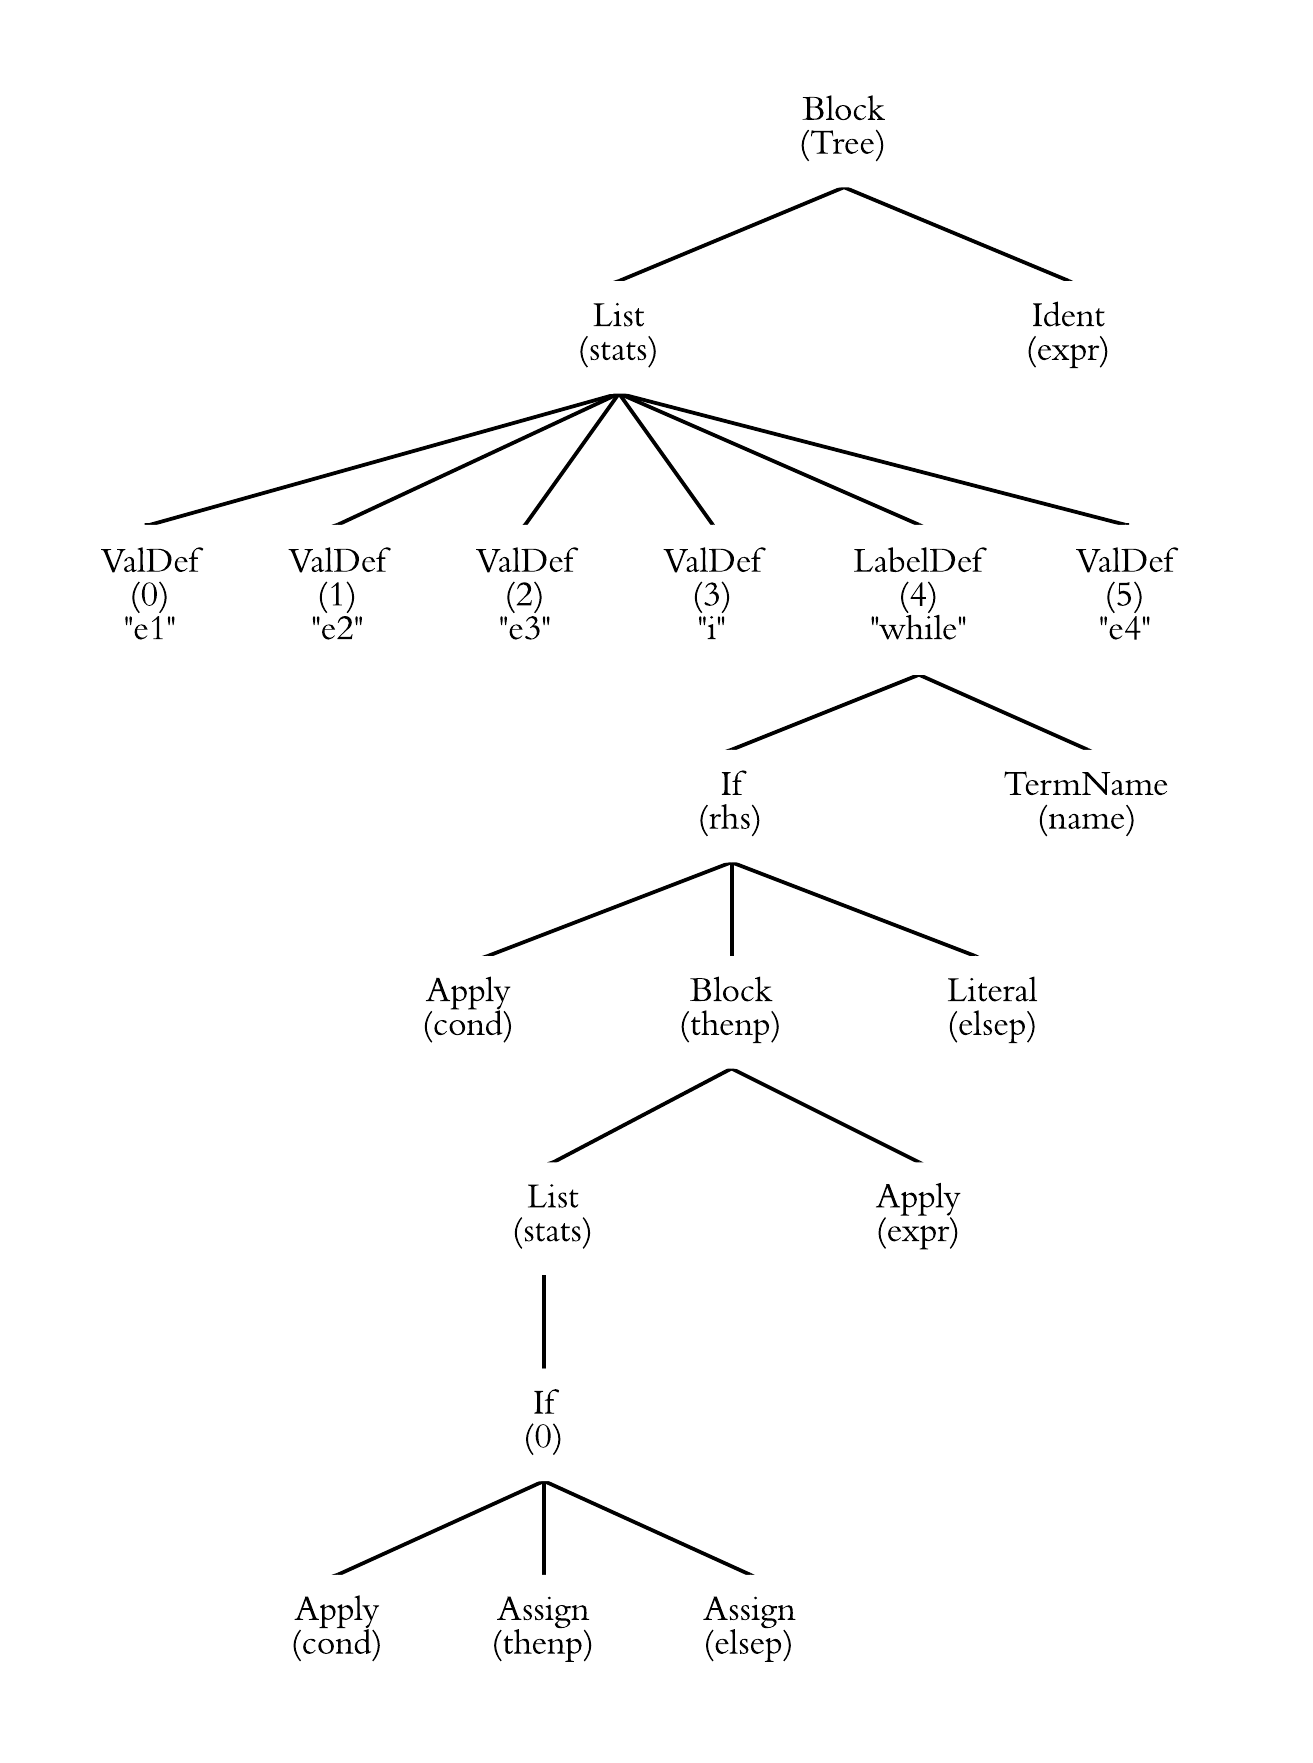
\includegraphics[width=0.8\linewidth]{figures/Tree}
\caption{Scala AST}
\label{fig:Tree}
\end{figure}

\section{CFG Definition}
The CFG is another intermediate representation that is produced from Scala AST in the first stage of the algorithm. Frances E. Allen \cite{allen1970control} defines a CFG as "a directed graph in which the nodes represent basic blocks and the edges represent control flow paths". CFG serves as framework for static analysis of program control flow. Many code generators partition intermediate representation instructions into basic blocks, which consist of sequences of instructions or statements that are always executed together \cite{lam2006compilers}. Basic blocks are a straight line, single-entry code with no branching except at the end of the sequence. 

\begin{figure}[h!]
\centering
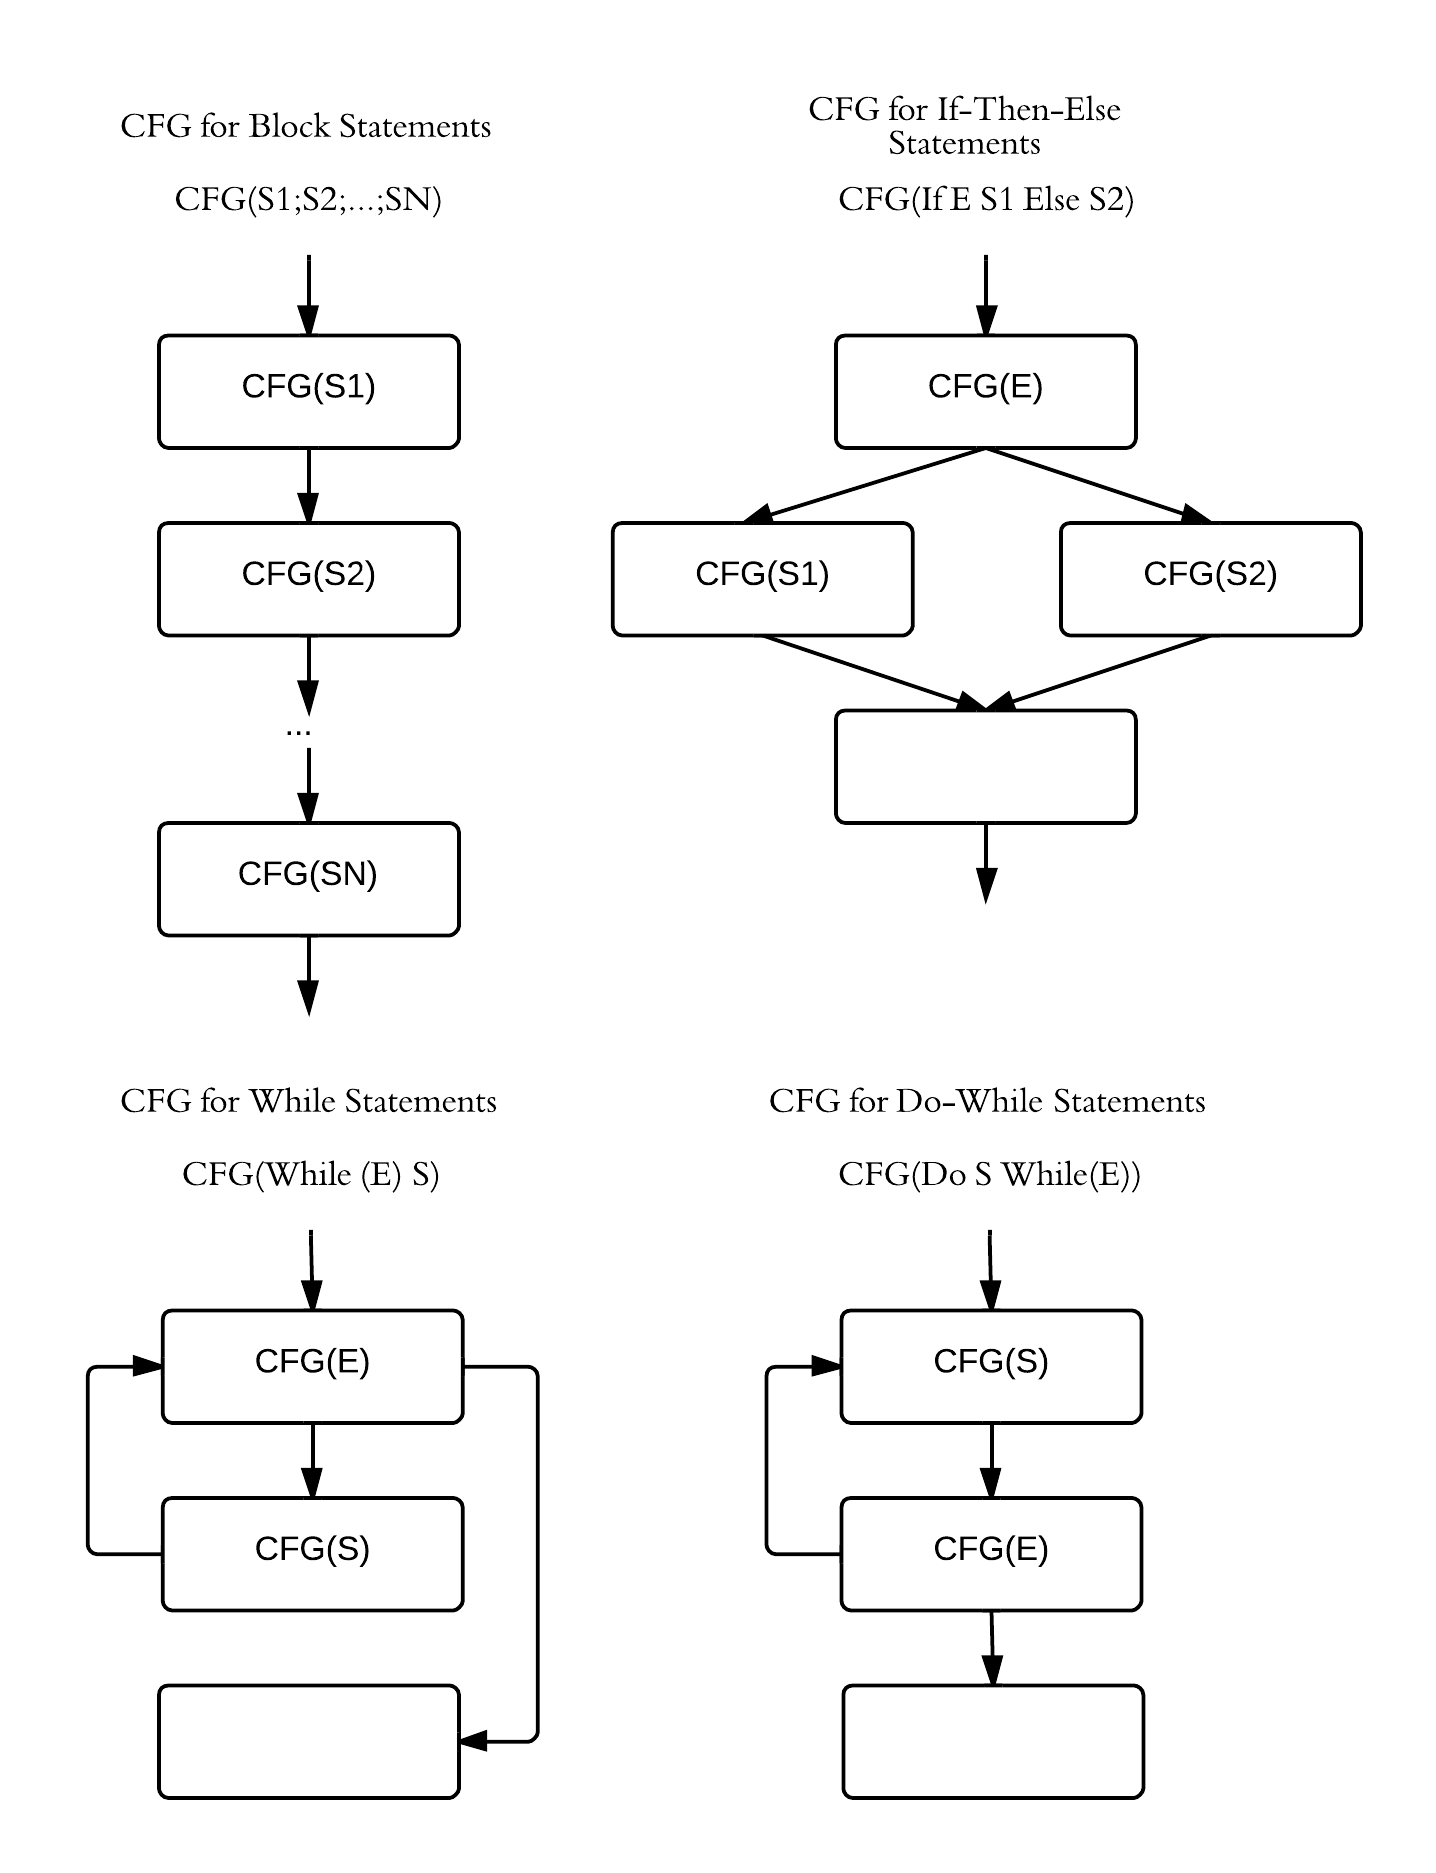
\includegraphics[width=0.7\linewidth]{figures/Graph}
\caption{CFG of Various Statements}
\label{fig:Graph}
\end{figure}

Edges represent possible flow of control from the end of one block to the beginning of the other. There may be multiple incoming or outgoing edges for each block \cite{allen1970control}. After the intermediate code has been partitioned into basic blocks, the flow of control between them can be represented by a CFG. There is an edge from block A to block B if and only if it is possible for the first statement in block B to immediately follow the last statement in block A. Given a Block statement, If-Then-Else statement, and While-statement, we formulate the expected CFG result from the first stage of the algorithm as shown in Figure 1.3. In the second stage of our algorithm, we analyze the graph to detect data dependencies and subsequently add another type of Edges which show the data dependencies between the nodes of the CFG. 

\section{Create CFG from AST Algorithm}
Creating CFG from AST is the first stage of the intermediate code and code generation process. This algorithm takes as an input a Scala AST and produces the output of a lower-level intermediate representation CFG $G=(V,E)$ with set $V$ of vertices and a set $E$ of directed edges. Each vertex $V$ is a sequence of one or multiple nodes $n$ in the AST. 

The idea is to traverse the tree from top to bottom starting from the $root$ and to visit each node $n$ of the children recursively. We check the type of each node $n$ and perform a set of actions accordingly. The procedure $createCFG(nCurr, G, vCurr, X)$ takes as input the following parameters. 
\begin{itemize}
\item $nCurr$ refers to the node that is currently being visited in the AST. In the beginning, $nCurr$ is initialized to root of the full AST of the program. Since we traverse the tree from top to bottom, the $nCurr$ becomes the root of the subtree of the initial root node. Depending on the type of the Tree, the $nCurr$ is either pushed to the current Vertex $vCurr$ or the subtree of the $nCurr$ is visited recursively. 

\item $G=(V,E)$ refers to the CFG produced by the procedure and is continuously being updated whenever recursion takes place. The CFG consists of a set of vertices and a set of directed edges. Each vertex of the resulted CFG is a sequence of statements or nodes in the AST. The vertices set $V$ of the graph has initial member of $vCurr$ whereas the edges set $E$ is initialized to an empty set.   

\item $vCurr$ refers to the vertex of the CFG that is currently being built. If the $nCurr$ or a subtree does not contain control flow or branches, the $nCurr$ will be pushed to the $vCurr$. Subsequently, if the subtree contains branches or control flow, new vertex will be added to the CFG as well as directed edges from the $vCurr$ to the new vertex. Furthermore, the new vertex will become the new $vCurr$ and the whole procedure of checking $nCurr$ for control flow is repeated. In the initialization, $vCurr$ is set to empty sequence since we just begin to traverse the tree. 

\item $X$ is a stack to store the variable which contains branches and needs to be updated with the return value of either the then part or the else part of the control flow. In the algorithm, this variable will be re-assigned to the return value and will be deleted from the stack allowing the stack empty at the end of the procedure.  

\end{itemize}

\begin{algorithm}[h]

\caption{Creating Control Flow Diagram from AST Part 1}\label{CFG}
\begin{algorithmic}[1]
\Initialize { $v_{curr}\gets [ ],V\gets \{v_{curr}\},E\gets \emptyset,X\gets [ ], n_{curr}\gets root$}
\Procedure{createCFG}{$n_{curr},G,v_{curr},X$}
\Switch {$n_{curr}$}
  \Case {$Block(stats,expr)$}
  	\For {each $s$ in $stats$}
  	\State $(G,v_{curr},X)\gets \Call{createCFG}{s,G, v_{curr},\emptyset}$
   	\EndFor  
    \State $(G,v_{curr},X)\gets \Call{createCFG}{expr,G, v_{curr},X}$
       	\State \textbf{return} $(G,v_{curr},X)$
      \EndCase
       
  \Case {$ValDef(name, rhs)$}
  		\If {$containsBranches(rhs)$}
  			\State $\Call{push}{ValDef(name,\emptyset),v_{curr}} $
  			\State $\Call{push}{name,X} $
  			\State $(G,v_{curr},X)\gets \Call{createCFG}{rhs,G, v_{curr},X} $
  		\Else
  			\State $\Call{push}{n_{curr}, v_{curr}} $
  		\EndIf
  	\State \textbf{return} $(G,v_{curr},X)$
  \EndCase

  \Case {$Assign(name,rhs)$}
    	\If {$containsBranches(rhs)$}
    		\State $\Call{push}{name,X} $
    		\State $(G,v_{curr},X)\gets \Call{createCFG}{rhs,G, v_{curr},X} $

    	\Else
    			\State $\Call{push}{n_{curr}, v_{curr}} $
    		\EndIf
    	\State \textbf{return} $(G,v_{curr},X)$
  \EndCase
  \Case {$While(cond,body)$}
  	\State $v_{condStart} \gets \Call{newV}$
  	\State $V \gets V \cup \{v_{condStart}\}; E \gets E \cup \{(v_{curr},v_{condStart})\}$ 
  	\State $(G,v_{condEnd},X)\gets \Call{createCFG}{cond,G,v_{condStart},\emptyset} $
  	\State $v_{bodyStart} \gets \Call{newV}{ }$
  	\State $V \gets V \cup \{v_{bodyStart}\}; E \gets E \cup \{(v_{condEnd},v_{bodyStart})\}$
  	\State $(G,v_{bodyEnd},X)\gets \Call{createCFG}{body,G, v_{bodyStart},\emptyset} $
  	\State $v_{curr} \gets \Call{newV}{ }$
  	\State $V \gets V \cup \{v_{curr}\}; E \gets E \cup \{(v_{condEnd},v_{curr}),(v_{bodyEnd},v_{condStart})\}$
  	\State \textbf{return} $(G,v_{curr},X)$
  \EndCase
 \algstore{bkbreak}
 \end{algorithmic}
 \end{algorithm}
 \begin{algorithm}
 \addtocounter{algorithm}{-1}
 \caption{Creating Control Flow Diagram from AST Part 2}\label{CFG2}
 \begin{algorithmic}[1]
 \algrestore{bkbreak}
  \Case {$DoWhile(cond,body)$}
      	\State $v_{bodyStart} \gets \Call{newV}{ }$
      	\State $V \gets V \cup \{v_{bodyStart}\}; E \gets E \cup \{(v_{curr},v_{bodyStart})\}$
  	\State $(G,v_{bodyEnd},X)\gets \Call{createCFG}{body,G, v_{body},\emptyset} $
  	\State $v_{condStart} \gets \Call{newV}{ }$
      	\State $V \gets V \cup \{v_{bodyEnd}, v_{condStart}\}; E \gets E \cup \{(v_{bodyEnd},v_{condStart})\}$ 
      	\State $(G,v_{condEnd},X)\gets \Call{createCFG}{cond,G,v_{cond},\emptyset} $
      	\State $v_{curr} \gets \Call{newV}{ }$
      	\State $V \gets V \cup \{v_{curr},v_{condEnd}\}$
      	\State $E \gets E \cup \{(v_{condEnd},v_{curr}),(v_{condEnd},v_{bodyStart})\}$
      	\State \textbf{return} $(G,v_{curr},X)$
    \EndCase
  \Case {$If(cond,thenp,elsep)$}
  	\State $(G,v_{cond},X)\gets \Call{createCFG}{cond,G, v_{cond},\emptyset}$
  	\State $v_{thenp} \gets \Call{newV}{ }$
  	\State $V \gets V \cup \{ v_{thenp}; E \gets E \cup \{(v_{curr},v_{thenp})\}$
  	\State $(G,v_{thenp},X)\gets \Call{createCFG}{thenp,G, v_{thenp},X} $
  	
  	\State $v_{elsep} \gets \Call{newV}{ }$
  	\State $V \gets V \cup \{v_{elsep}\};E \gets E \cup \{(v_{curr},v_{elsep})$
  	\State $(G,v_{elsep},X)\gets \Call{createCFG}{elsep,G, v_{elsep},X} $
  	
  	\State $v_{curr} \gets \Call{newV}{ }$
  	\State $V \gets V \cup \{v_{curr}\};E \gets E \cup \{(v_{thenp},v_{curr}),(v_{elsep},v_{curr})\}$
 	  	
  	\State \textbf{return} $(G,v_{curr},X)$
    	
  \EndCase

  \Case { $\_$}
  	\If {$X \neq \emptyset$}
	\State $name \gets X.head$
  	\State $\Call{push}{Assign(name,n_{curr}),v_{curr}} $ 
  	\Else
  	\State $\Call{push}{n_{curr},v_{curr}} $ 
  	\EndIf 
  	\State \textbf{return} $(G,v_{curr},X)$
  	
  \EndCase
 
\EndSwitch
\EndProcedure
\Procedure{containsBranches}{$n_{curr}$}
\Switch {$n_{curr}$}
  \Case {$Block(_,expr)$}
  \State $\Call{containsBranches}{expr}$
  \EndCase
  \Case {$If(\_)$}
  	\State \textbf{return} $true$
  \EndCase
  \Case {$\_$}
    \State \textbf{return} $false$
    \EndCase
\EndSwitch
\EndProcedure
\end{algorithmic}
\end{algorithm}

Using Scala pattern matching, we are able to traverse the tree and match the current node of the tree $nCurr$ to a Scala AST type. Based on its type, the following procedure will be taken. 

\begin{itemize}

\item $Block(stats, expr)$.
A Block typically consists of a list of statements and an expression. For every statement inside the Block, the procedure is called recursively and the Graph $G=(V,E)$, current vertex $vCurr$, and stack of variable $X$ are subsequently updated. After each statement is visited, the procedure is also called recursively for the single expression.  

\item $ValDef(name,rhs)$
As mentioned in the Scala AST introduction section, ValDef refers to definition of a variable both immutable (val) and mutable (var). In this case, we check whether the ValDef contains branches or control flow. If there is a control flow inside the ValDef, the same ValDef with a mutable identifier is pushed to the current vertex $vCurr$ and the name of the variable of type TermName is stored in the stack variable $X$. The name of the variable needs to be stored because it must be assigned later on with the value in the Then part or the Else part of the control flow. The rhs then becomes the current node $nCurr$ and the procedure is called recursively.  Sample program that will encounter this case is provided in the Listing 1.3 below. In this case, the variable $e3$ is stored in $X$ and later will be assigned to the function "e1.map {..}" or function "e2.map {..}".
\begin{lstlisting}[language=scala,caption=ValDef with Branches, label = valdef]
val e3 = if (e1.map(x => x._2).reduce((x, y) => Math.max(x, y)).fetch().head > 50)
	e1.map { x => (x._1, x._2 + 1000, x._3)}
else
	e2.map { x => (x._1, x._2 + 1500, x._3)}
\end{lstlisting}

If the ValDef does not contain branches, then the current node $nCurr$ is simply pushed to the current vertex $vCurr$. 

\item $Assign(name,rhs)$
The procedure for the case Assign is similar with ValDef. We check whether the tree or node contains branches. If it does, the name of the variable is stored in the stack variable $X$ to be assigned later on with the value in the Then part or the Else part of the control flow. The procedure is then called recursively with the rhs as the new current node $nCurr$. Similar to ValDef, if the Tree does not contain branches, the current node $nCurr$ is simply pushed to the current vertex $vCurr$.

\item $While(cond,body)$
As depicted in Figure 2-3, for While loop, a new vertex $vCondStart$ is created to store the condition of the iteration. A directed edge is defined from the current vertex $vCurr$ to the new vertex $vCondStart$. A new vertex $vBodyStart$ is also created to store the statements in the $body$ of the iteration. Both the $cond$ and $body$ may or may not contain branches. Hence, recursive call both for $cond$ and $body$ take place which results in the new vertex $vCondEnd$ and $vBodyEnd$ respectively. A directed edge is defined from the end of the $body$ which is the vertex $vBodyEnd$ to the beginning of the $cond$ which is the vertex $vCondStart$. At the end, a new vertex is created as the new current vertex $vCurr$ and a directed edge is defined from the vertex $vBodyEnd$ to the new current vertex $vCurr$. 

\item $DoWhile(cond,body)$
The procedure for DoWhile case is similar with While case with the differences in the order the vertices are created as well as the directed edges connecting the vertices. The $vBodyStart$ is created first and is connected to the $vCurr$. The vertex result of the recursive call to the body of the iteration, vertex $vBodyEnd$ is connected to the new vertex $vCondStart$ which stores the condition of the iteration. The end of the condition $vCondEnd$ is connected to the start of the $body$ $vBodyStart$. Similar to the While loop, at the end, a new vertex is created as the new current vertex $vCurr$ and a directed edge is defined from the vertex $vCondEnd$ to the new current vertex $vCurr$. 

\item $If(cond,thenp,elsep)$
At first, we create a new vertex $vCond$ to store the condition of the If statement. A directed edge is connected from the current vertex $vCurr$ to the $vCond$. A recursive call is performed to the procedure since the $cond$ may or may not contain branches. We then create two new vertices $vThenp$ and $vElsep$ to represent the Then part and the Else part of the If statement consecutively. A directed edge is defined from $vCond$ to both new vertices $vThenp$ and $vElsep$ to represent all possible flows. Recursive call is performed both for the Then part $thenp$ and Else part $elsep$ since they may or may not contain branches. At the end, a new vertex is created as the new current vertex $vCurr$ and a directed edge is defined both from the vertex $vThenp$ and vertex $vElsep$ to the new current vertex $vCurr$. 

\item $Default Case)$
We first check whether the stack of variable $X$ contains any member. If yes, then we have get the last member inserted to $X$ which is a name, and assign the current node $nCurr$ to the name. This assignment is then pushed to the current vertex $vCurr$. If the stack variable $X$ does not contain any member, which means no assignment is needed, the current node $nCurr$ is simply pushed to the current vertex $vCurr$. 
\end{itemize}

We perform this algorithm with the input of the Scala AST of the program in Listing 2-1. The CFG result is shown in Figure 1.4. 

\begin{figure}[h!]
\centering
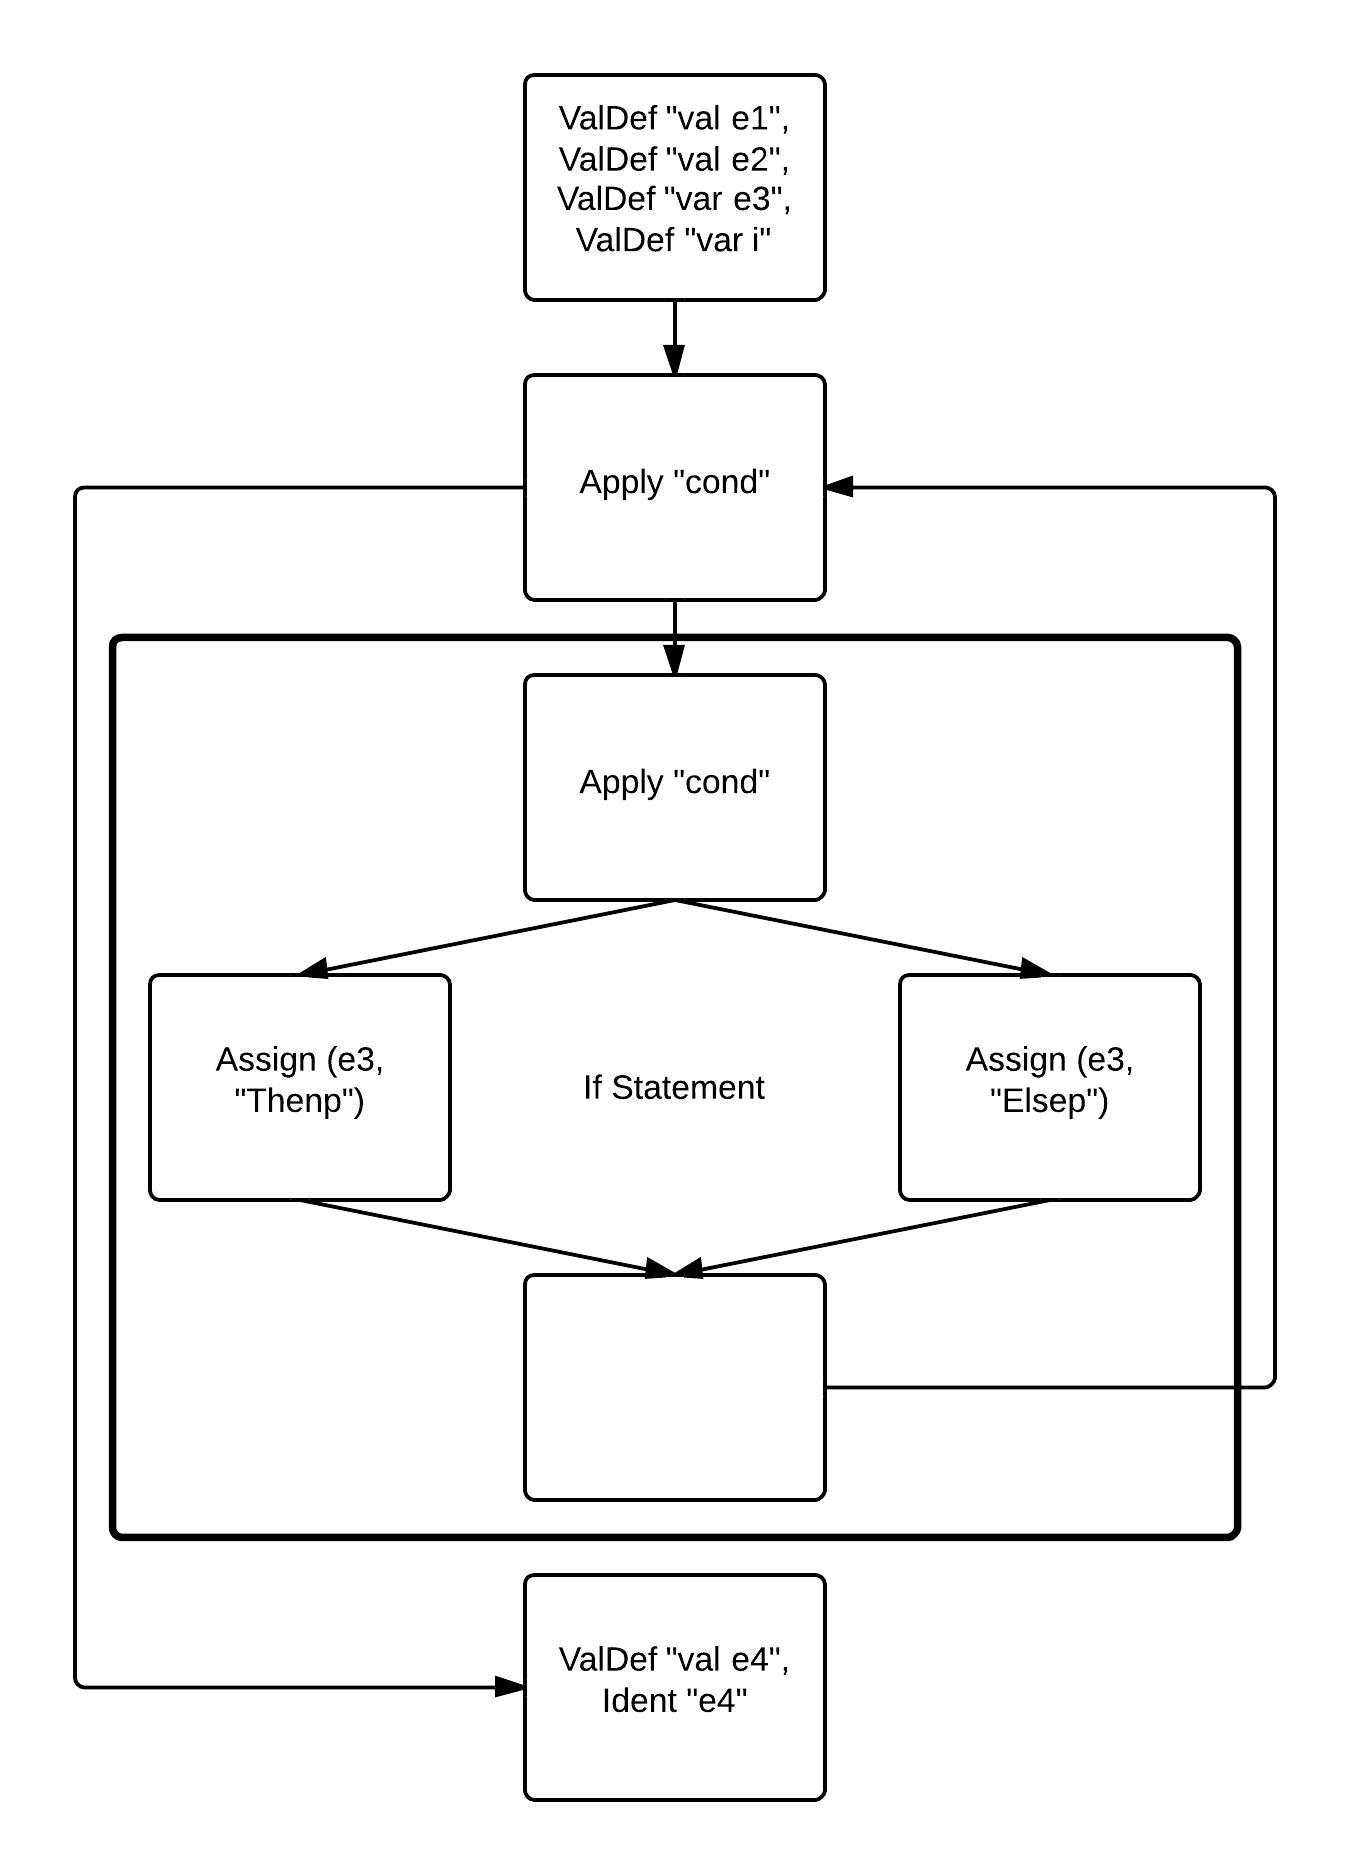
\includegraphics[width=0.7\linewidth]{figures/FinalGraph}
\caption{CFG of Scala AST of sample Program}
\label{fig:FinalGraph}
\end{figure}



